% -*- root: ../gvoysey-thesis.tex -*-
\chapter{Results}
\label{chapter:Results}
\thispagestyle{myheadings}

% set this to the location of the figures for this chapter. it may
% also want to be ../Figures/2_Body/ or something. make sure that
% it has a trailing directory separator (i.e., '/')!
\graphicspath{{5_Results/Figures/}}
\section{Chapter Summary} % (fold)
\label{sec:results_summary}
This chapter describes the results obtained when using the modeling environment described in~\autoref{chapter:Methods} to simulate a series of tone-in-noise experiments performed in humans by \citeauthor{Mehraei2016Auditory} to elucidate certain aspects of cochlear synaptopathy. 

% section results_summary (end)
\section{Tone in noise experiment} % (fold)
\label{sec:tone_in_noise}

\subsection{Stimuli} % (fold)
\label{sub:stimuli}
Following \citeauthor{Mehraei2015Auditory,Mehraei2016Auditory}, 6 stimului were programmatically generated and stored as WAV files with a sampling frequency of 100 kHz.  As shown in \autoref{fig:stimuli-used}, stimulus onset was delayed by 20 $\mu$s of silence, and then consisted of 80 dB SPL clicks with a repetition rate of 100 ms in the presence of gaussian noise at different signal to noise ratios. 

\begin{figure}[htbp]
	\centering
	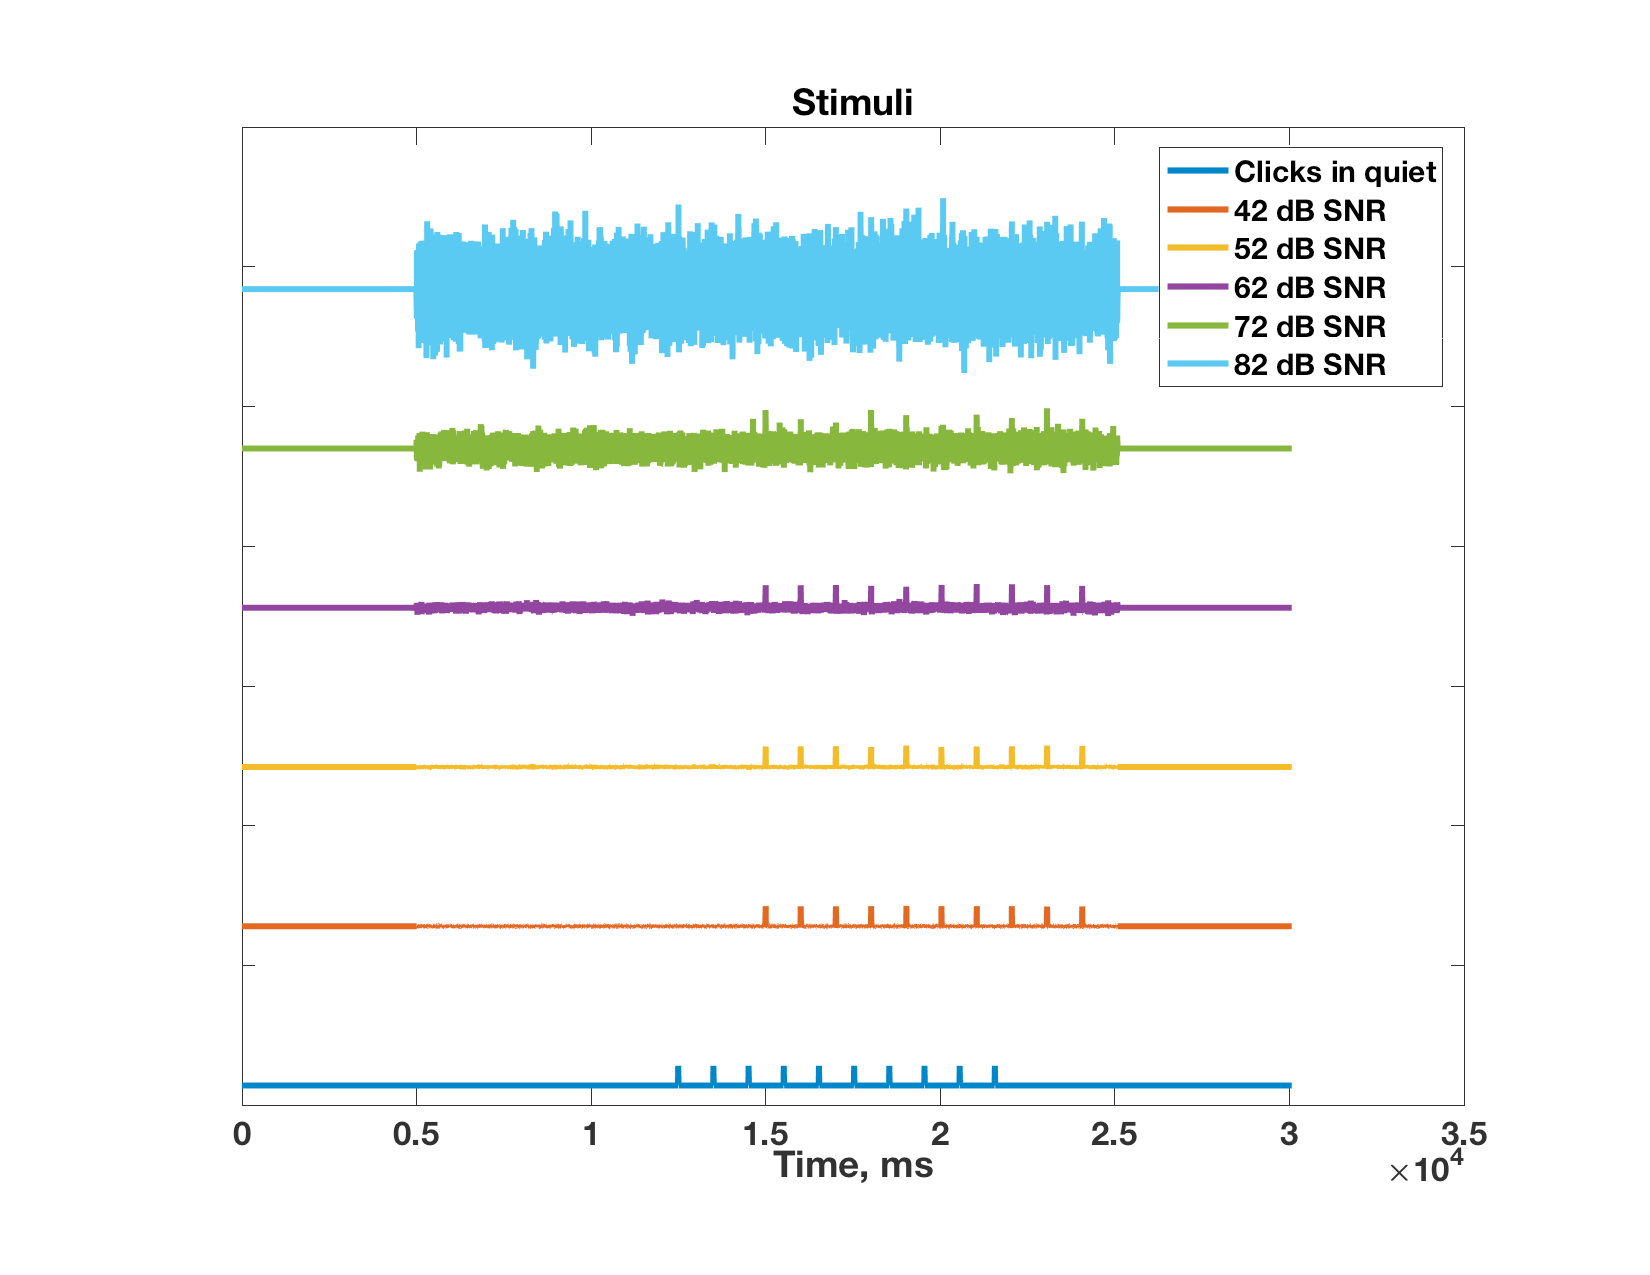
\includegraphics[width=0.95\textwidth]{stimuli-used.pdf}
	\caption[Experimental Stimuli]{Stimuli used to drive the auditory models.}
	\label{fig:stimuli-used}
\end{figure}
% subsection stimuli (end)

\begin{itemize}
	\item Ran the same stimului used by~\cite{Mehraei2015Auditory}: 80dB click, varying SNR
	\item Ran 1208 model configurations which varied  the stimulus SNR, the level and type of synaptopathy applied to the results, which peripheral model was used, whether the BM had any cf-weighting, and which brainstem model was used. 
	\item used a python library and cluster resources to make sure the results are easily searchable. 
	\item roughly 400 GB of model results.
	\item Can now examine the effects of individual parameter changes. 
	\item can now compare results to both prior modeling results and human data. 
\end{itemize}


\section{Simulations}
The experiment design tool described in \autoref{sec:automated_parameter_exploration} was used to specify a range of values for each parameter in Corti to reveal the relative contributions of each. 

In total, 240 separate simulations were run in parallel on Boston University's high-performance computing cluster over the course of approximately 9 days.  Model output was automatically stored into a HDF5 database approximately 250 GB in size.

\section{Effect of peripheral model} % (fold)
\label{sec:effect_of_peripheral_model}
The verhulst and zilany models will produce different estimates of the auditory nerve response. Prior work had their results very different; with recent changes to the verhulst model, this may have changed.
% section effect_of_peripheral_model (end)

\section{Effect of Synaptopathy} % (fold)
\label{sec:effect_of_synaptopathy}
Six kinds of synaptopathy were simulated: uniform and low-- and medium--SR specific losses of 10, 25, and 50 percent of each fiber type. 
% section effect_of_synaptopathy (end)

\section{Effect of CF weighting} % (fold)
\label{sec:effect_of_cf_weighting}
In models of the periphery that include more low SR fibers at high frequencies, synaptopathic losses will change.
% section effect_of_cf_weighting (end)

\section{Effect of brainstem model} % (fold)
\label{sec:effect_of_brainstem_model}
Does our intuition about a more physiologicaly relevant brainstem and midbrain model capturing more of the diversity of human responses bear out? 
% section effect_of_brainstem_model (end)